\documentclass[twoside]{book}

% Packages required by doxygen
\usepackage{calc}
\usepackage{doxygen}
\usepackage{graphicx}
\usepackage[utf8]{inputenc}
\usepackage{makeidx}
\usepackage{multicol}
\usepackage{multirow}
\usepackage{textcomp}
\usepackage[table]{xcolor}

% Font selection
\usepackage[T1]{fontenc}
\usepackage{mathptmx}
\usepackage[scaled=.90]{helvet}
\usepackage{courier}
\usepackage{amssymb}
\usepackage{sectsty}
\renewcommand{\familydefault}{\sfdefault}
\allsectionsfont{%
  \fontseries{bc}\selectfont%
  \color{darkgray}%
}
\renewcommand{\DoxyLabelFont}{%
  \fontseries{bc}\selectfont%
  \color{darkgray}%
}

% Page & text layout
\usepackage{geometry}
\geometry{%
  a4paper,%
  top=2.5cm,%
  bottom=2.5cm,%
  left=2.5cm,%
  right=2.5cm%
}
\tolerance=750
\hfuzz=15pt
\hbadness=750
\setlength{\emergencystretch}{15pt}
\setlength{\parindent}{0cm}
\setlength{\parskip}{0.2cm}
\makeatletter
\renewcommand{\paragraph}{%
  \@startsection{paragraph}{4}{0ex}{-1.0ex}{1.0ex}{%
    \normalfont\normalsize\bfseries\SS@parafont%
  }%
}
\renewcommand{\subparagraph}{%
  \@startsection{subparagraph}{5}{0ex}{-1.0ex}{1.0ex}{%
    \normalfont\normalsize\bfseries\SS@subparafont%
  }%
}
\makeatother

% Headers & footers
\usepackage{fancyhdr}
\pagestyle{fancyplain}
\fancyhead[LE]{\fancyplain{}{\bfseries\thepage}}
\fancyhead[CE]{\fancyplain{}{}}
\fancyhead[RE]{\fancyplain{}{\bfseries\leftmark}}
\fancyhead[LO]{\fancyplain{}{\bfseries\rightmark}}
\fancyhead[CO]{\fancyplain{}{}}
\fancyhead[RO]{\fancyplain{}{\bfseries\thepage}}
\fancyfoot[LE]{\fancyplain{}{}}
\fancyfoot[CE]{\fancyplain{}{}}
\fancyfoot[RE]{\fancyplain{}{\bfseries\scriptsize Generated on Mon May 27 2013 15:08:51 for Quest For Fire by Doxygen }}
\fancyfoot[LO]{\fancyplain{}{\bfseries\scriptsize Generated on Mon May 27 2013 15:08:51 for Quest For Fire by Doxygen }}
\fancyfoot[CO]{\fancyplain{}{}}
\fancyfoot[RO]{\fancyplain{}{}}
\renewcommand{\footrulewidth}{0.4pt}
\renewcommand{\chaptermark}[1]{%
  \markboth{#1}{}%
}
\renewcommand{\sectionmark}[1]{%
  \markright{\thesection\ #1}%
}

% Indices & bibliography
\usepackage{natbib}
\usepackage[titles]{tocloft}
\setcounter{tocdepth}{3}
\setcounter{secnumdepth}{5}
\makeindex

% Hyperlinks (required, but should be loaded last)
\usepackage{ifpdf}
\ifpdf
  \usepackage[pdftex,pagebackref=true]{hyperref}
\else
  \usepackage[ps2pdf,pagebackref=true]{hyperref}
\fi
\hypersetup{%
  colorlinks=true,%
  linkcolor=blue,%
  citecolor=blue,%
  unicode%
}

% Custom commands
\newcommand{\clearemptydoublepage}{%
  \newpage{\pagestyle{empty}\cleardoublepage}%
}


%===== C O N T E N T S =====

\begin{document}

% Titlepage & ToC
\hypersetup{pageanchor=false}
\pagenumbering{roman}
\begin{titlepage}
\vspace*{7cm}
\begin{center}%
{\Large Quest For Fire }\\
\vspace*{1cm}
{\large Generated by Doxygen 1.8.4}\\
\vspace*{0.5cm}
{\small Mon May 27 2013 15:08:51}\\
\end{center}
\end{titlepage}
\clearemptydoublepage
\tableofcontents
\clearemptydoublepage
\pagenumbering{arabic}
\hypersetup{pageanchor=true}

%--- Begin generated contents ---
\chapter{Hierarchical Index}
\section{Class Hierarchy}
This inheritance list is sorted roughly, but not completely, alphabetically\-:\begin{DoxyCompactList}
\item \contentsline{section}{Gameplay\-Object}{\pageref{da/df6/classGameplayObject}}{}
\begin{DoxyCompactList}
\item \contentsline{section}{Troglodyte}{\pageref{dd/d4c/classTroglodyte}}{}
\end{DoxyCompactList}
\item \contentsline{section}{Gameplay\-Objects\-List}{\pageref{d9/d30/classGameplayObjectsList}}{}
\item \contentsline{section}{Main}{\pageref{db/d4a/classMain}}{}
\item \contentsline{section}{Order}{\pageref{d5/d6b/classOrder}}{}
\item \contentsline{section}{Player}{\pageref{d2/d4b/classPlayer}}{}
\item Runnable\begin{DoxyCompactList}
\item \contentsline{section}{Game\-Logic}{\pageref{dd/d20/classGameLogic}}{}
\item \contentsline{section}{Map\-Panel}{\pageref{d3/dab/classMapPanel}}{}
\end{DoxyCompactList}
\item \contentsline{section}{Squadron}{\pageref{d3/d9e/classSquadron}}{}
\item J\-Frame\begin{DoxyCompactList}
\item \contentsline{section}{Game\-Window}{\pageref{d3/dce/classGameWindow}}{}
\end{DoxyCompactList}
\item J\-Panel\begin{DoxyCompactList}
\item \contentsline{section}{Map\-Panel}{\pageref{d3/dab/classMapPanel}}{}
\end{DoxyCompactList}
\end{DoxyCompactList}

\chapter{Class Index}
\section{Class List}
Here are the classes, structs, unions and interfaces with brief descriptions\-:\begin{DoxyCompactList}
\item\contentsline{section}{\hyperlink{classGameLogic}{Game\-Logic} }{\pageref{dd/d20/classGameLogic}}{}
\item\contentsline{section}{\hyperlink{classGameplayObject}{Gameplay\-Object} }{\pageref{da/df6/classGameplayObject}}{}
\item\contentsline{section}{\hyperlink{classGameplayObjectsList}{Gameplay\-Objects\-List} }{\pageref{d9/d30/classGameplayObjectsList}}{}
\item\contentsline{section}{\hyperlink{classGameWindow}{Game\-Window} }{\pageref{d3/dce/classGameWindow}}{}
\item\contentsline{section}{\hyperlink{classMain}{Main} }{\pageref{db/d4a/classMain}}{}
\item\contentsline{section}{\hyperlink{classMapPanel}{Map\-Panel} }{\pageref{d3/dab/classMapPanel}}{}
\item\contentsline{section}{\hyperlink{classOrder}{Order} }{\pageref{d5/d6b/classOrder}}{}
\item\contentsline{section}{\hyperlink{classPlayer}{Player} }{\pageref{d2/d4b/classPlayer}}{}
\item\contentsline{section}{\hyperlink{classSquadron}{Squadron} }{\pageref{d3/d9e/classSquadron}}{}
\item\contentsline{section}{\hyperlink{classTroglodyte}{Troglodyte} }{\pageref{dd/d4c/classTroglodyte}}{}
\end{DoxyCompactList}

\chapter{File Index}
\section{File List}
Here is a list of all files with brief descriptions\-:\begin{DoxyCompactList}
\item\contentsline{section}{src/\hyperlink{GameLogic_8java}{Game\-Logic.\-java} }{\pageref{de/dff/GameLogic_8java}}{}
\item\contentsline{section}{src/\hyperlink{GameplayObject_8java}{Gameplay\-Object.\-java} }{\pageref{d9/d56/GameplayObject_8java}}{}
\item\contentsline{section}{src/\hyperlink{GameplayObjectsList_8java}{Gameplay\-Objects\-List.\-java} }{\pageref{dd/dcd/GameplayObjectsList_8java}}{}
\item\contentsline{section}{src/\hyperlink{GameWindow_8java}{Game\-Window.\-java} }{\pageref{de/d08/GameWindow_8java}}{}
\item\contentsline{section}{src/\hyperlink{Main_8java}{Main.\-java} }{\pageref{d6/d13/Main_8java}}{}
\item\contentsline{section}{src/\hyperlink{MapPanel_8java}{Map\-Panel.\-java} }{\pageref{dc/d40/MapPanel_8java}}{}
\item\contentsline{section}{src/\hyperlink{Order_8java}{Order.\-java} }{\pageref{d2/dc6/Order_8java}}{}
\item\contentsline{section}{src/\hyperlink{Player_8java}{Player.\-java} }{\pageref{d4/d01/Player_8java}}{}
\item\contentsline{section}{src/\hyperlink{Squadron_8java}{Squadron.\-java} }{\pageref{d7/d87/Squadron_8java}}{}
\item\contentsline{section}{src/\hyperlink{Troglodyte_8java}{Troglodyte.\-java} }{\pageref{db/d13/Troglodyte_8java}}{}
\end{DoxyCompactList}

\chapter{Class Documentation}
\hypertarget{classGameLogic}{\section{Game\-Logic Class Reference}
\label{classGameLogic}\index{Game\-Logic@{Game\-Logic}}
}
Inheritance diagram for Game\-Logic\-:\begin{figure}[H]
\begin{center}
\leavevmode
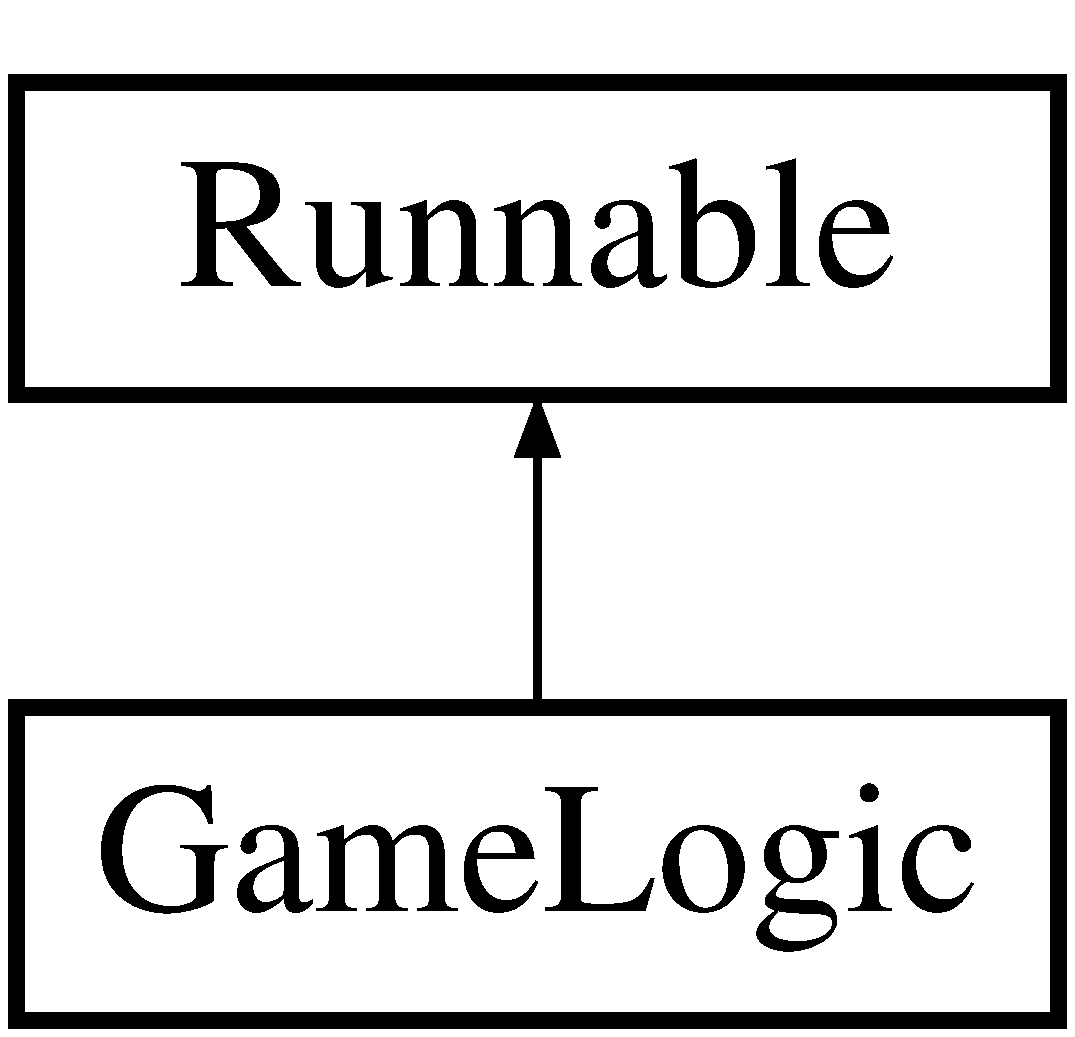
\includegraphics[height=2.000000cm]{dd/d20/classGameLogic}
\end{center}
\end{figure}
\subsection*{Public Member Functions}
\begin{DoxyCompactItemize}
\item 
boolean \hyperlink{classGameLogic_a3c8aac57f25ae1d7d83144a22b6a6569}{running} ()
\item 
void \hyperlink{classGameLogic_a5c8a5055ff4a003a255bcdf52cbd4d2c}{Start} ()
\item 
void \hyperlink{classGameLogic_a53f9f036abbff3736a0d2bed33198b06}{Stop} ()
\item 
void \hyperlink{classGameLogic_a3a00031f831728a8073b58229e3d23c4}{create\-Troglodyte} ()
\item 
void \hyperlink{classGameLogic_a51ad9cef9c4414961b2f025bf659c068}{run} ()
\end{DoxyCompactItemize}
\subsection*{Private Attributes}
\begin{DoxyCompactItemize}
\item 
Thread \hyperlink{classGameLogic_a63998de862313caa158c414ad3a8dad0}{worker}
\item 
Semaphore \hyperlink{classGameLogic_a09c53c7f1a59ad90cd34966360edddcc}{main\-Sync}
\item 
volatile \hyperlink{classGameplayObjectsList}{Gameplay\-Objects\-List} \hyperlink{classGameLogic_a48be08c7f3371c4e6fc68aaf6c839afe}{objects\-List}
\item 
volatile boolean \hyperlink{classGameLogic_af6686d787ae2639adc84f522f332c3ee}{running}
\item 
Random \hyperlink{classGameLogic_a1b940a2b65f42fdee9ee1fb7a910b1d2}{ran}
\end{DoxyCompactItemize}
\subsection*{Static Private Attributes}
\begin{DoxyCompactItemize}
\item 
static final int \hyperlink{classGameLogic_ad140b2df5a64378f6039ba1f683f6b9f}{speed} = 50
\end{DoxyCompactItemize}


\subsection{Member Function Documentation}
\hypertarget{classGameLogic_a3a00031f831728a8073b58229e3d23c4}{\index{Game\-Logic@{Game\-Logic}!create\-Troglodyte@{create\-Troglodyte}}
\index{create\-Troglodyte@{create\-Troglodyte}!GameLogic@{Game\-Logic}}
\subsubsection[{create\-Troglodyte}]{\setlength{\rightskip}{0pt plus 5cm}void Game\-Logic.\-create\-Troglodyte (
\begin{DoxyParamCaption}
{}
\end{DoxyParamCaption}
)}}\label{classGameLogic_a3a00031f831728a8073b58229e3d23c4}
\hypertarget{classGameLogic_a51ad9cef9c4414961b2f025bf659c068}{\index{Game\-Logic@{Game\-Logic}!run@{run}}
\index{run@{run}!GameLogic@{Game\-Logic}}
\subsubsection[{run}]{\setlength{\rightskip}{0pt plus 5cm}void Game\-Logic.\-run (
\begin{DoxyParamCaption}
{}
\end{DoxyParamCaption}
)}}\label{classGameLogic_a51ad9cef9c4414961b2f025bf659c068}
Główna pętla logiki gry.\hypertarget{classGameLogic_a3c8aac57f25ae1d7d83144a22b6a6569}{\index{Game\-Logic@{Game\-Logic}!running@{running}}
\index{running@{running}!GameLogic@{Game\-Logic}}
\subsubsection[{running}]{\setlength{\rightskip}{0pt plus 5cm}boolean Game\-Logic.\-running (
\begin{DoxyParamCaption}
{}
\end{DoxyParamCaption}
)}}\label{classGameLogic_a3c8aac57f25ae1d7d83144a22b6a6569}
\hypertarget{classGameLogic_a5c8a5055ff4a003a255bcdf52cbd4d2c}{\index{Game\-Logic@{Game\-Logic}!Start@{Start}}
\index{Start@{Start}!GameLogic@{Game\-Logic}}
\subsubsection[{Start}]{\setlength{\rightskip}{0pt plus 5cm}void Game\-Logic.\-Start (
\begin{DoxyParamCaption}
{}
\end{DoxyParamCaption}
)}}\label{classGameLogic_a5c8a5055ff4a003a255bcdf52cbd4d2c}
\hypertarget{classGameLogic_a53f9f036abbff3736a0d2bed33198b06}{\index{Game\-Logic@{Game\-Logic}!Stop@{Stop}}
\index{Stop@{Stop}!GameLogic@{Game\-Logic}}
\subsubsection[{Stop}]{\setlength{\rightskip}{0pt plus 5cm}void Game\-Logic.\-Stop (
\begin{DoxyParamCaption}
{}
\end{DoxyParamCaption}
)}}\label{classGameLogic_a53f9f036abbff3736a0d2bed33198b06}
Gdy zażądano przerwania gry. Ta metoda może być wywołana również przez dowolny panel.

\subsection{Member Data Documentation}
\hypertarget{classGameLogic_a09c53c7f1a59ad90cd34966360edddcc}{\index{Game\-Logic@{Game\-Logic}!main\-Sync@{main\-Sync}}
\index{main\-Sync@{main\-Sync}!GameLogic@{Game\-Logic}}
\subsubsection[{main\-Sync}]{\setlength{\rightskip}{0pt plus 5cm}Semaphore Game\-Logic.\-main\-Sync\hspace{0.3cm}{\ttfamily [private]}}}\label{classGameLogic_a09c53c7f1a59ad90cd34966360edddcc}
\hypertarget{classGameLogic_a48be08c7f3371c4e6fc68aaf6c839afe}{\index{Game\-Logic@{Game\-Logic}!objects\-List@{objects\-List}}
\index{objects\-List@{objects\-List}!GameLogic@{Game\-Logic}}
\subsubsection[{objects\-List}]{\setlength{\rightskip}{0pt plus 5cm}volatile {\bf Gameplay\-Objects\-List} Game\-Logic.\-objects\-List\hspace{0.3cm}{\ttfamily [private]}}}\label{classGameLogic_a48be08c7f3371c4e6fc68aaf6c839afe}
\hypertarget{classGameLogic_a1b940a2b65f42fdee9ee1fb7a910b1d2}{\index{Game\-Logic@{Game\-Logic}!ran@{ran}}
\index{ran@{ran}!GameLogic@{Game\-Logic}}
\subsubsection[{ran}]{\setlength{\rightskip}{0pt plus 5cm}Random Game\-Logic.\-ran\hspace{0.3cm}{\ttfamily [private]}}}\label{classGameLogic_a1b940a2b65f42fdee9ee1fb7a910b1d2}
\hypertarget{classGameLogic_af6686d787ae2639adc84f522f332c3ee}{\index{Game\-Logic@{Game\-Logic}!running@{running}}
\index{running@{running}!GameLogic@{Game\-Logic}}
\subsubsection[{running}]{\setlength{\rightskip}{0pt plus 5cm}volatile boolean Game\-Logic.\-running\hspace{0.3cm}{\ttfamily [private]}}}\label{classGameLogic_af6686d787ae2639adc84f522f332c3ee}
\hypertarget{classGameLogic_ad140b2df5a64378f6039ba1f683f6b9f}{\index{Game\-Logic@{Game\-Logic}!speed@{speed}}
\index{speed@{speed}!GameLogic@{Game\-Logic}}
\subsubsection[{speed}]{\setlength{\rightskip}{0pt plus 5cm}final int Game\-Logic.\-speed = 50\hspace{0.3cm}{\ttfamily [static]}, {\ttfamily [private]}}}\label{classGameLogic_ad140b2df5a64378f6039ba1f683f6b9f}
\hypertarget{classGameLogic_a63998de862313caa158c414ad3a8dad0}{\index{Game\-Logic@{Game\-Logic}!worker@{worker}}
\index{worker@{worker}!GameLogic@{Game\-Logic}}
\subsubsection[{worker}]{\setlength{\rightskip}{0pt plus 5cm}Thread Game\-Logic.\-worker\hspace{0.3cm}{\ttfamily [private]}}}\label{classGameLogic_a63998de862313caa158c414ad3a8dad0}
Klasa zarządzająca logiką gry. 

The documentation for this class was generated from the following file\-:\begin{DoxyCompactItemize}
\item 
src/\hyperlink{GameLogic_8java}{Game\-Logic.\-java}\end{DoxyCompactItemize}

\hypertarget{classGameplayObject}{\section{Gameplay\-Object Class Reference}
\label{classGameplayObject}\index{Gameplay\-Object@{Gameplay\-Object}}
}
Inheritance diagram for Gameplay\-Object\-:\begin{figure}[H]
\begin{center}
\leavevmode
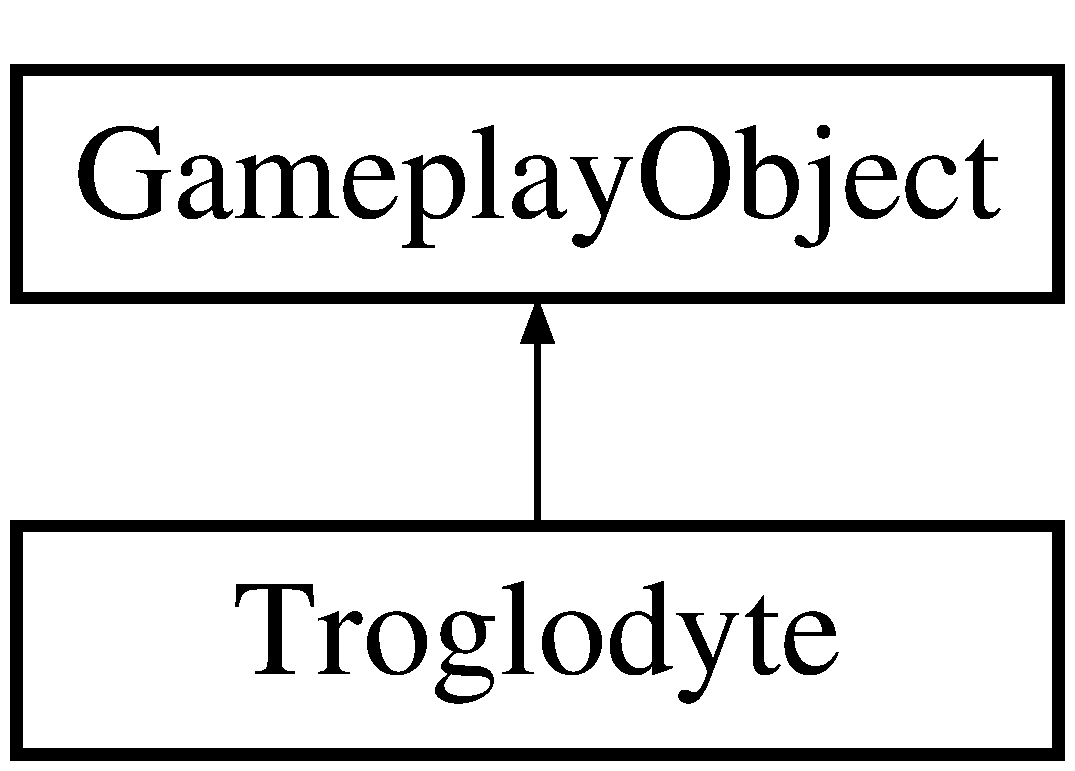
\includegraphics[height=2.000000cm]{da/df6/classGameplayObject}
\end{center}
\end{figure}
\subsection*{Public Member Functions}
\begin{DoxyCompactItemize}
\item 
String \hyperlink{classGameplayObject_ab0356b4a3f2d8a89f44fa8ae5389b764}{get\-Name} ()
\item 
void \hyperlink{classGameplayObject_a1af215eb801ca7acb2e143d60c5f26b2}{set\-Visible} (boolean \hyperlink{classGameplayObject_ad33ca23e562d57352dffda8631b15909}{visible})
\item 
boolean \hyperlink{classGameplayObject_ac533926c9b2fb82d8a7d47d7a5dbff4d}{is\-Visible} ()
\item 
abstract void \hyperlink{classGameplayObject_ad99f71d67a42e68dad3f923adc8a2699}{place} (int x, int y)
\item 
abstract void \hyperlink{classGameplayObject_ad0e03d54842aa2bb721648ad702ef350}{draw} (Graphics2\-D g)
\end{DoxyCompactItemize}
\subsection*{Private Attributes}
\begin{DoxyCompactItemize}
\item 
boolean \hyperlink{classGameplayObject_ad33ca23e562d57352dffda8631b15909}{visible}
\item 
String \hyperlink{classGameplayObject_a0b0fe50720b6ea4dc9261295cdfb7a0c}{name}
\end{DoxyCompactItemize}


\subsection{Member Function Documentation}
\hypertarget{classGameplayObject_ad0e03d54842aa2bb721648ad702ef350}{\index{Gameplay\-Object@{Gameplay\-Object}!draw@{draw}}
\index{draw@{draw}!GameplayObject@{Gameplay\-Object}}
\subsubsection[{draw}]{\setlength{\rightskip}{0pt plus 5cm}abstract void Gameplay\-Object.\-draw (
\begin{DoxyParamCaption}
\item[{Graphics2\-D}]{g}
\end{DoxyParamCaption}
)\hspace{0.3cm}{\ttfamily [pure virtual]}}}\label{classGameplayObject_ad0e03d54842aa2bb721648ad702ef350}


Implemented in \hyperlink{classTroglodyte_ace39490a0220ea11ca717e479c761e0d}{Troglodyte}.

\hypertarget{classGameplayObject_ab0356b4a3f2d8a89f44fa8ae5389b764}{\index{Gameplay\-Object@{Gameplay\-Object}!get\-Name@{get\-Name}}
\index{get\-Name@{get\-Name}!GameplayObject@{Gameplay\-Object}}
\subsubsection[{get\-Name}]{\setlength{\rightskip}{0pt plus 5cm}String Gameplay\-Object.\-get\-Name (
\begin{DoxyParamCaption}
{}
\end{DoxyParamCaption}
)}}\label{classGameplayObject_ab0356b4a3f2d8a89f44fa8ae5389b764}
\hypertarget{classGameplayObject_ac533926c9b2fb82d8a7d47d7a5dbff4d}{\index{Gameplay\-Object@{Gameplay\-Object}!is\-Visible@{is\-Visible}}
\index{is\-Visible@{is\-Visible}!GameplayObject@{Gameplay\-Object}}
\subsubsection[{is\-Visible}]{\setlength{\rightskip}{0pt plus 5cm}boolean Gameplay\-Object.\-is\-Visible (
\begin{DoxyParamCaption}
{}
\end{DoxyParamCaption}
)}}\label{classGameplayObject_ac533926c9b2fb82d8a7d47d7a5dbff4d}
\hypertarget{classGameplayObject_ad99f71d67a42e68dad3f923adc8a2699}{\index{Gameplay\-Object@{Gameplay\-Object}!place@{place}}
\index{place@{place}!GameplayObject@{Gameplay\-Object}}
\subsubsection[{place}]{\setlength{\rightskip}{0pt plus 5cm}abstract void Gameplay\-Object.\-place (
\begin{DoxyParamCaption}
\item[{int}]{x, }
\item[{int}]{y}
\end{DoxyParamCaption}
)\hspace{0.3cm}{\ttfamily [pure virtual]}}}\label{classGameplayObject_ad99f71d67a42e68dad3f923adc8a2699}


Implemented in \hyperlink{classTroglodyte_a8dced6c4c8542fd20eb58e05f4ee96d1}{Troglodyte}.

\hypertarget{classGameplayObject_a1af215eb801ca7acb2e143d60c5f26b2}{\index{Gameplay\-Object@{Gameplay\-Object}!set\-Visible@{set\-Visible}}
\index{set\-Visible@{set\-Visible}!GameplayObject@{Gameplay\-Object}}
\subsubsection[{set\-Visible}]{\setlength{\rightskip}{0pt plus 5cm}void Gameplay\-Object.\-set\-Visible (
\begin{DoxyParamCaption}
\item[{boolean}]{visible}
\end{DoxyParamCaption}
)}}\label{classGameplayObject_a1af215eb801ca7acb2e143d60c5f26b2}


\subsection{Member Data Documentation}
\hypertarget{classGameplayObject_a0b0fe50720b6ea4dc9261295cdfb7a0c}{\index{Gameplay\-Object@{Gameplay\-Object}!name@{name}}
\index{name@{name}!GameplayObject@{Gameplay\-Object}}
\subsubsection[{name}]{\setlength{\rightskip}{0pt plus 5cm}String Gameplay\-Object.\-name\hspace{0.3cm}{\ttfamily [private]}}}\label{classGameplayObject_a0b0fe50720b6ea4dc9261295cdfb7a0c}
\hypertarget{classGameplayObject_ad33ca23e562d57352dffda8631b15909}{\index{Gameplay\-Object@{Gameplay\-Object}!visible@{visible}}
\index{visible@{visible}!GameplayObject@{Gameplay\-Object}}
\subsubsection[{visible}]{\setlength{\rightskip}{0pt plus 5cm}boolean Gameplay\-Object.\-visible\hspace{0.3cm}{\ttfamily [private]}}}\label{classGameplayObject_ad33ca23e562d57352dffda8631b15909}


The documentation for this class was generated from the following file\-:\begin{DoxyCompactItemize}
\item 
src/\hyperlink{GameplayObject_8java}{Gameplay\-Object.\-java}\end{DoxyCompactItemize}

\hypertarget{classGameplayObjectsList}{\section{Gameplay\-Objects\-List Class Reference}
\label{classGameplayObjectsList}\index{Gameplay\-Objects\-List@{Gameplay\-Objects\-List}}
}
\subsection*{Public Member Functions}
\begin{DoxyCompactItemize}
\item 
void \hyperlink{classGameplayObjectsList_a184ca546acf5b2a6f6212d188c526814}{reset\-Pointer} ()
\item 
void \hyperlink{classGameplayObjectsList_a79d161d85c0207a0d2821e616ee03b9e}{add\-Game\-Object} (\hyperlink{classGameplayObject}{Gameplay\-Object} gpo)
\item 
void \hyperlink{classGameplayObjectsList_aa4e9ea9384811fa31b2c602f5a767446}{del\-Game\-Object} (\hyperlink{classGameplayObject}{Gameplay\-Object} gpo)
\item 
\hyperlink{classGameplayObject}{Gameplay\-Object} \hyperlink{classGameplayObjectsList_af4d3baabb227c988807c086e48ed43a7}{get\-By\-Name} (String name)
\item 
\hyperlink{classGameplayObject}{Gameplay\-Object} \hyperlink{classGameplayObjectsList_a3a882b2fbc9d668bfdfc0ba689955eab}{next} ()
\item 
\hyperlink{classGameplayObject}{Gameplay\-Object} \hyperlink{classGameplayObjectsList_ac0f9be5825684a3973192a1405084b82}{next\-Visible} ()
\end{DoxyCompactItemize}
\subsection*{Private Attributes}
\begin{DoxyCompactItemize}
\item 
Linked\-List$<$ \hyperlink{classGameplayObject}{Gameplay\-Object} $>$ \hyperlink{classGameplayObjectsList_ae07f69f02fab6b47e861477fad9b6749}{objects\-List}
\item 
int \hyperlink{classGameplayObjectsList_a21dae4e14c5c6f1e211dce81ef133129}{pointer}
\end{DoxyCompactItemize}


\subsection{Member Function Documentation}
\hypertarget{classGameplayObjectsList_a79d161d85c0207a0d2821e616ee03b9e}{\index{Gameplay\-Objects\-List@{Gameplay\-Objects\-List}!add\-Game\-Object@{add\-Game\-Object}}
\index{add\-Game\-Object@{add\-Game\-Object}!GameplayObjectsList@{Gameplay\-Objects\-List}}
\subsubsection[{add\-Game\-Object}]{\setlength{\rightskip}{0pt plus 5cm}void Gameplay\-Objects\-List.\-add\-Game\-Object (
\begin{DoxyParamCaption}
\item[{{\bf Gameplay\-Object}}]{gpo}
\end{DoxyParamCaption}
)}}\label{classGameplayObjectsList_a79d161d85c0207a0d2821e616ee03b9e}
\hypertarget{classGameplayObjectsList_aa4e9ea9384811fa31b2c602f5a767446}{\index{Gameplay\-Objects\-List@{Gameplay\-Objects\-List}!del\-Game\-Object@{del\-Game\-Object}}
\index{del\-Game\-Object@{del\-Game\-Object}!GameplayObjectsList@{Gameplay\-Objects\-List}}
\subsubsection[{del\-Game\-Object}]{\setlength{\rightskip}{0pt plus 5cm}void Gameplay\-Objects\-List.\-del\-Game\-Object (
\begin{DoxyParamCaption}
\item[{{\bf Gameplay\-Object}}]{gpo}
\end{DoxyParamCaption}
)}}\label{classGameplayObjectsList_aa4e9ea9384811fa31b2c602f5a767446}
\hypertarget{classGameplayObjectsList_af4d3baabb227c988807c086e48ed43a7}{\index{Gameplay\-Objects\-List@{Gameplay\-Objects\-List}!get\-By\-Name@{get\-By\-Name}}
\index{get\-By\-Name@{get\-By\-Name}!GameplayObjectsList@{Gameplay\-Objects\-List}}
\subsubsection[{get\-By\-Name}]{\setlength{\rightskip}{0pt plus 5cm}{\bf Gameplay\-Object} Gameplay\-Objects\-List.\-get\-By\-Name (
\begin{DoxyParamCaption}
\item[{String}]{name}
\end{DoxyParamCaption}
)}}\label{classGameplayObjectsList_af4d3baabb227c988807c086e48ed43a7}
\hypertarget{classGameplayObjectsList_a3a882b2fbc9d668bfdfc0ba689955eab}{\index{Gameplay\-Objects\-List@{Gameplay\-Objects\-List}!next@{next}}
\index{next@{next}!GameplayObjectsList@{Gameplay\-Objects\-List}}
\subsubsection[{next}]{\setlength{\rightskip}{0pt plus 5cm}{\bf Gameplay\-Object} Gameplay\-Objects\-List.\-next (
\begin{DoxyParamCaption}
{}
\end{DoxyParamCaption}
)}}\label{classGameplayObjectsList_a3a882b2fbc9d668bfdfc0ba689955eab}
\hypertarget{classGameplayObjectsList_ac0f9be5825684a3973192a1405084b82}{\index{Gameplay\-Objects\-List@{Gameplay\-Objects\-List}!next\-Visible@{next\-Visible}}
\index{next\-Visible@{next\-Visible}!GameplayObjectsList@{Gameplay\-Objects\-List}}
\subsubsection[{next\-Visible}]{\setlength{\rightskip}{0pt plus 5cm}{\bf Gameplay\-Object} Gameplay\-Objects\-List.\-next\-Visible (
\begin{DoxyParamCaption}
{}
\end{DoxyParamCaption}
)}}\label{classGameplayObjectsList_ac0f9be5825684a3973192a1405084b82}
\hypertarget{classGameplayObjectsList_a184ca546acf5b2a6f6212d188c526814}{\index{Gameplay\-Objects\-List@{Gameplay\-Objects\-List}!reset\-Pointer@{reset\-Pointer}}
\index{reset\-Pointer@{reset\-Pointer}!GameplayObjectsList@{Gameplay\-Objects\-List}}
\subsubsection[{reset\-Pointer}]{\setlength{\rightskip}{0pt plus 5cm}void Gameplay\-Objects\-List.\-reset\-Pointer (
\begin{DoxyParamCaption}
{}
\end{DoxyParamCaption}
)}}\label{classGameplayObjectsList_a184ca546acf5b2a6f6212d188c526814}


\subsection{Member Data Documentation}
\hypertarget{classGameplayObjectsList_ae07f69f02fab6b47e861477fad9b6749}{\index{Gameplay\-Objects\-List@{Gameplay\-Objects\-List}!objects\-List@{objects\-List}}
\index{objects\-List@{objects\-List}!GameplayObjectsList@{Gameplay\-Objects\-List}}
\subsubsection[{objects\-List}]{\setlength{\rightskip}{0pt plus 5cm}Linked\-List$<${\bf Gameplay\-Object}$>$ Gameplay\-Objects\-List.\-objects\-List\hspace{0.3cm}{\ttfamily [private]}}}\label{classGameplayObjectsList_ae07f69f02fab6b47e861477fad9b6749}
\hypertarget{classGameplayObjectsList_a21dae4e14c5c6f1e211dce81ef133129}{\index{Gameplay\-Objects\-List@{Gameplay\-Objects\-List}!pointer@{pointer}}
\index{pointer@{pointer}!GameplayObjectsList@{Gameplay\-Objects\-List}}
\subsubsection[{pointer}]{\setlength{\rightskip}{0pt plus 5cm}int Gameplay\-Objects\-List.\-pointer\hspace{0.3cm}{\ttfamily [private]}}}\label{classGameplayObjectsList_a21dae4e14c5c6f1e211dce81ef133129}


The documentation for this class was generated from the following file\-:\begin{DoxyCompactItemize}
\item 
src/\hyperlink{GameplayObjectsList_8java}{Gameplay\-Objects\-List.\-java}\end{DoxyCompactItemize}

\hypertarget{classGameWindow}{\section{Game\-Window Class Reference}
\label{classGameWindow}\index{Game\-Window@{Game\-Window}}
}
Inheritance diagram for Game\-Window\-:\begin{figure}[H]
\begin{center}
\leavevmode
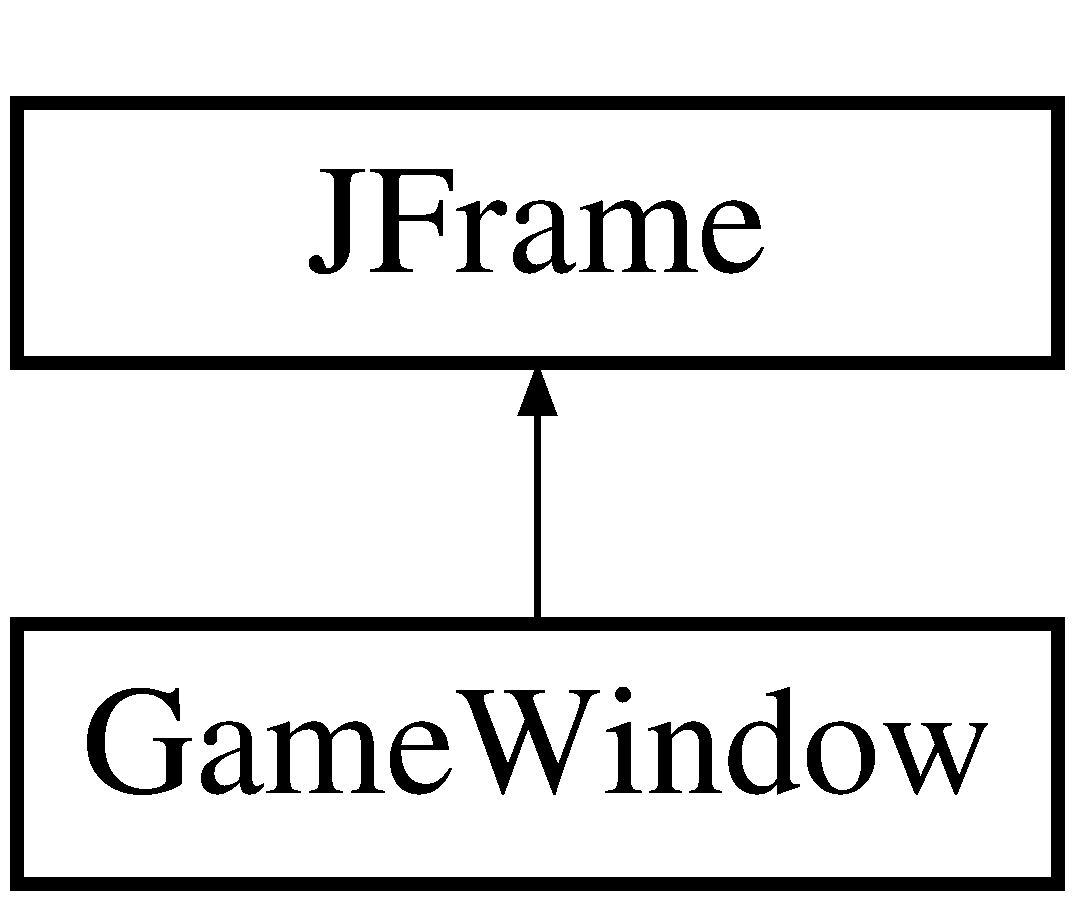
\includegraphics[height=2.000000cm]{d3/dce/classGameWindow}
\end{center}
\end{figure}
\subsection*{Public Member Functions}
\begin{DoxyCompactItemize}
\item 
void \hyperlink{classGameWindow_a94d5bf99fbc4d6e6e15897ce3babadae}{Start} ()
\end{DoxyCompactItemize}
\subsection*{Private Attributes}
\begin{DoxyCompactItemize}
\item 
\hyperlink{classGameLogic}{Game\-Logic} \hyperlink{classGameWindow_afdc585949ce286ac31b620d4680e4a40}{game\-Logic}
\item 
\hyperlink{classMapPanel}{Map\-Panel} \hyperlink{classGameWindow_a6695d85b00f5b75982b4e0afe8b49149}{map\-Panel}
\item 
Semaphore \hyperlink{classGameWindow_abb7ba8d8b4b506372e17a1f5c523ca6b}{panel\-Semaphore}
\item 
volatile \hyperlink{classGameplayObjectsList}{Gameplay\-Objects\-List} \hyperlink{classGameWindow_acd0adf7ae69050f844a07b90f4891536}{objects\-List}
\end{DoxyCompactItemize}
\subsection*{Static Private Attributes}
\begin{DoxyCompactItemize}
\item 
static final long \hyperlink{classGameWindow_a29133b2b32da4e6fc4c63ea6438c6050}{serial\-Version\-U\-I\-D} = -\/7712354877306446942\-L
\item 
static String \hyperlink{classGameWindow_aca5fe59b0761d6873e1d7b48cd37ea8c}{title} = \char`\"{}Quest for Fire\char`\"{}
\end{DoxyCompactItemize}


\subsection{Member Function Documentation}
\hypertarget{classGameWindow_a94d5bf99fbc4d6e6e15897ce3babadae}{\index{Game\-Window@{Game\-Window}!Start@{Start}}
\index{Start@{Start}!GameWindow@{Game\-Window}}
\subsubsection[{Start}]{\setlength{\rightskip}{0pt plus 5cm}void Game\-Window.\-Start (
\begin{DoxyParamCaption}
{}
\end{DoxyParamCaption}
)}}\label{classGameWindow_a94d5bf99fbc4d6e6e15897ce3babadae}


\subsection{Member Data Documentation}
\hypertarget{classGameWindow_afdc585949ce286ac31b620d4680e4a40}{\index{Game\-Window@{Game\-Window}!game\-Logic@{game\-Logic}}
\index{game\-Logic@{game\-Logic}!GameWindow@{Game\-Window}}
\subsubsection[{game\-Logic}]{\setlength{\rightskip}{0pt plus 5cm}{\bf Game\-Logic} Game\-Window.\-game\-Logic\hspace{0.3cm}{\ttfamily [private]}}}\label{classGameWindow_afdc585949ce286ac31b620d4680e4a40}
\hypertarget{classGameWindow_a6695d85b00f5b75982b4e0afe8b49149}{\index{Game\-Window@{Game\-Window}!map\-Panel@{map\-Panel}}
\index{map\-Panel@{map\-Panel}!GameWindow@{Game\-Window}}
\subsubsection[{map\-Panel}]{\setlength{\rightskip}{0pt plus 5cm}{\bf Map\-Panel} Game\-Window.\-map\-Panel\hspace{0.3cm}{\ttfamily [private]}}}\label{classGameWindow_a6695d85b00f5b75982b4e0afe8b49149}
\hypertarget{classGameWindow_acd0adf7ae69050f844a07b90f4891536}{\index{Game\-Window@{Game\-Window}!objects\-List@{objects\-List}}
\index{objects\-List@{objects\-List}!GameWindow@{Game\-Window}}
\subsubsection[{objects\-List}]{\setlength{\rightskip}{0pt plus 5cm}volatile {\bf Gameplay\-Objects\-List} Game\-Window.\-objects\-List\hspace{0.3cm}{\ttfamily [private]}}}\label{classGameWindow_acd0adf7ae69050f844a07b90f4891536}
\hypertarget{classGameWindow_abb7ba8d8b4b506372e17a1f5c523ca6b}{\index{Game\-Window@{Game\-Window}!panel\-Semaphore@{panel\-Semaphore}}
\index{panel\-Semaphore@{panel\-Semaphore}!GameWindow@{Game\-Window}}
\subsubsection[{panel\-Semaphore}]{\setlength{\rightskip}{0pt plus 5cm}Semaphore Game\-Window.\-panel\-Semaphore\hspace{0.3cm}{\ttfamily [private]}}}\label{classGameWindow_abb7ba8d8b4b506372e17a1f5c523ca6b}
\hypertarget{classGameWindow_a29133b2b32da4e6fc4c63ea6438c6050}{\index{Game\-Window@{Game\-Window}!serial\-Version\-U\-I\-D@{serial\-Version\-U\-I\-D}}
\index{serial\-Version\-U\-I\-D@{serial\-Version\-U\-I\-D}!GameWindow@{Game\-Window}}
\subsubsection[{serial\-Version\-U\-I\-D}]{\setlength{\rightskip}{0pt plus 5cm}final long Game\-Window.\-serial\-Version\-U\-I\-D = -\/7712354877306446942\-L\hspace{0.3cm}{\ttfamily [static]}, {\ttfamily [private]}}}\label{classGameWindow_a29133b2b32da4e6fc4c63ea6438c6050}
\hypertarget{classGameWindow_aca5fe59b0761d6873e1d7b48cd37ea8c}{\index{Game\-Window@{Game\-Window}!title@{title}}
\index{title@{title}!GameWindow@{Game\-Window}}
\subsubsection[{title}]{\setlength{\rightskip}{0pt plus 5cm}String Game\-Window.\-title = \char`\"{}Quest for Fire\char`\"{}\hspace{0.3cm}{\ttfamily [static]}, {\ttfamily [private]}}}\label{classGameWindow_aca5fe59b0761d6873e1d7b48cd37ea8c}


The documentation for this class was generated from the following file\-:\begin{DoxyCompactItemize}
\item 
src/\hyperlink{GameWindow_8java}{Game\-Window.\-java}\end{DoxyCompactItemize}

\hypertarget{classMain}{\section{Main Class Reference}
\label{classMain}\index{Main@{Main}}
}
\subsection*{Static Public Member Functions}
\begin{DoxyCompactItemize}
\item 
static void \hyperlink{classMain_a8a5d0f827edddff706cc0e6740d0579a}{main} (String\mbox{[}$\,$\mbox{]} args)
\end{DoxyCompactItemize}
\subsection*{Static Private Attributes}
\begin{DoxyCompactItemize}
\item 
static \hyperlink{classGameplayObjectsList}{Gameplay\-Objects\-List} \hyperlink{classMain_a3e22bc113001df13ed3e382d7bf2284c}{objects\-List}
\end{DoxyCompactItemize}


\subsection{Member Function Documentation}
\hypertarget{classMain_a8a5d0f827edddff706cc0e6740d0579a}{\index{Main@{Main}!main@{main}}
\index{main@{main}!Main@{Main}}
\subsubsection[{main}]{\setlength{\rightskip}{0pt plus 5cm}static void Main.\-main (
\begin{DoxyParamCaption}
\item[{String\mbox{[}$\,$\mbox{]}}]{args}
\end{DoxyParamCaption}
)\hspace{0.3cm}{\ttfamily [static]}}}\label{classMain_a8a5d0f827edddff706cc0e6740d0579a}


\subsection{Member Data Documentation}
\hypertarget{classMain_a3e22bc113001df13ed3e382d7bf2284c}{\index{Main@{Main}!objects\-List@{objects\-List}}
\index{objects\-List@{objects\-List}!Main@{Main}}
\subsubsection[{objects\-List}]{\setlength{\rightskip}{0pt plus 5cm}{\bf Gameplay\-Objects\-List} Main.\-objects\-List\hspace{0.3cm}{\ttfamily [static]}, {\ttfamily [private]}}}\label{classMain_a3e22bc113001df13ed3e382d7bf2284c}

\begin{DoxyParams}{Parameters}
{\em args} & Główna klasa tworząca wątki i zarządzająca grą. \\
\hline
\end{DoxyParams}


The documentation for this class was generated from the following file\-:\begin{DoxyCompactItemize}
\item 
src/\hyperlink{Main_8java}{Main.\-java}\end{DoxyCompactItemize}

\hypertarget{classMapPanel}{\section{Map\-Panel Class Reference}
\label{classMapPanel}\index{Map\-Panel@{Map\-Panel}}
}
Inheritance diagram for Map\-Panel\-:\begin{figure}[H]
\begin{center}
\leavevmode
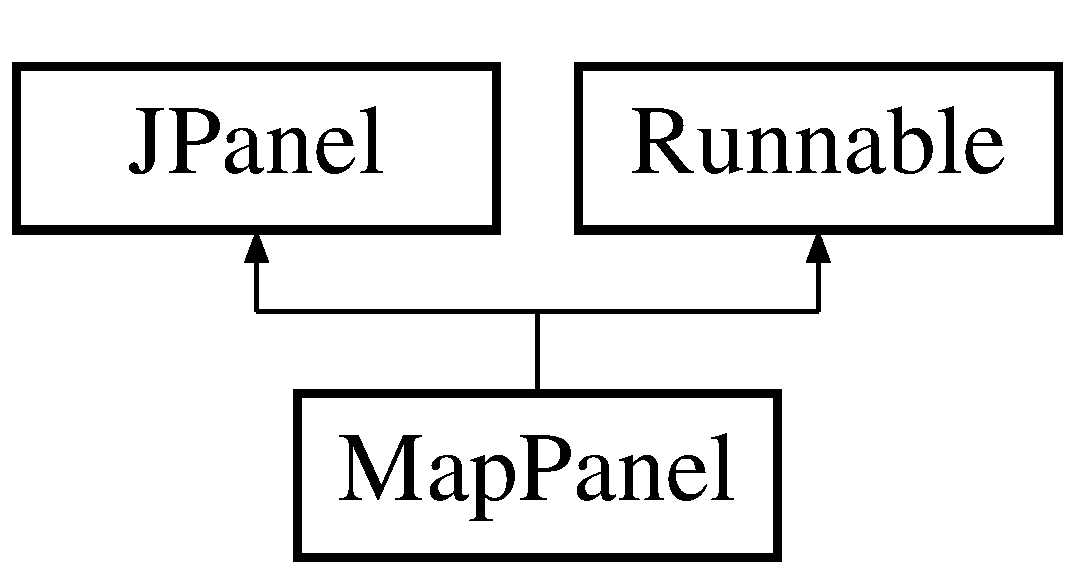
\includegraphics[height=2.000000cm]{d3/dab/classMapPanel}
\end{center}
\end{figure}
\subsection*{Public Member Functions}
\begin{DoxyCompactItemize}
\item 
void \hyperlink{classMapPanel_a7c1a269fe83ad8865f49bcb0155a4131}{add\-Notify} ()
\item 
void \hyperlink{classMapPanel_a5a1d201167de7399668e110c0f75c9be}{paint\-Component} (Graphics2\-D g)
\item 
void \hyperlink{classMapPanel_a6ae73cdac59708713354a2ba4f81aab0}{resume\-Game} ()
\item 
void \hyperlink{classMapPanel_a5efc48884233516e77d25d2e467913a6}{pause\-Game} ()
\item 
void \hyperlink{classMapPanel_a1bfb13628206b010c607a51461a5714e}{stop\-Game} ()
\item 
void \hyperlink{classMapPanel_ad3aa911c03a0e80f6a223b8f8eff43d6}{game\-Over} ()
\item 
void \hyperlink{classMapPanel_ad8cf61431c3e5928aeab0e1035fefe18}{run} ()
\end{DoxyCompactItemize}
\subsection*{Private Member Functions}
\begin{DoxyCompactItemize}
\item 
void \hyperlink{classMapPanel_add873c163ad14ab4e194ae9a897333b7}{set\-Controls} ()
\item 
void \hyperlink{classMapPanel_a51c4a598e2a1e0e385a4dd4bf4492e8e}{test\-Press} (int x, int y)
\item 
void \hyperlink{classMapPanel_a31f00f5993c4d117ba795d6ba46cb8a6}{game\-Update} ()
\item 
void \hyperlink{classMapPanel_a855596851c23f07b2a8e57e17e47cfb2}{game\-Render} ()
\item 
void \hyperlink{classMapPanel_aa04a6dded4624d9c3da9d136d35aff98}{paint\-Screen} ()
\item 
void \hyperlink{classMapPanel_ab700710546b15759204beddaddd26843}{start\-Game} ()
\end{DoxyCompactItemize}
\subsection*{Private Attributes}
\begin{DoxyCompactItemize}
\item 
Thread \hyperlink{classMapPanel_a2f4861c001b00d173bbad5573eb7fda7}{animator}
\item 
boolean \hyperlink{classMapPanel_a2af536efa9e8a4df2d0bef98b427a878}{running}
\item 
volatile boolean \hyperlink{classMapPanel_afaa79c91a69c6ce1e1edd062e066da06}{game\-Over} = false
\item 
Graphics2\-D \hyperlink{classMapPanel_ad691832c9f6f90db5bed90f359ce46fc}{dbg}
\item 
Image \hyperlink{classMapPanel_aad322f3de5764d74d0da0ee2862e1da4}{db\-Image} = null
\item 
\hyperlink{classGameLogic}{Game\-Logic} \hyperlink{classMapPanel_a2ea62977a77f6de53552a52d7f99bb9e}{game\-Logic}
\item 
Semaphore \hyperlink{classMapPanel_a94fbd1f030f19c4f0841defc21fe81b2}{semaphore}
\item 
volatile \hyperlink{classGameplayObjectsList}{Gameplay\-Objects\-List} \hyperlink{classMapPanel_a636653ac7ebbff9faf60f89bfb3887ab}{objects\-List}
\end{DoxyCompactItemize}
\subsection*{Static Private Attributes}
\begin{DoxyCompactItemize}
\item 
static final long \hyperlink{classMapPanel_a63b76f204807ce3eefbe8e01a80359d6}{serial\-Version\-U\-I\-D} = 1794571289521271349\-L
\item 
static final int \hyperlink{classMapPanel_a78dbdc3c4f055e777934bf965835ecdc}{P\-W\-I\-D\-T\-H} = 600
\item 
static final int \hyperlink{classMapPanel_ab568855b8c5789ced1e76c48046c1775}{P\-H\-E\-I\-G\-H\-T} = 400
\item 
static final int \hyperlink{classMapPanel_ac8a10b9f2d89e400c0b9ad615459a35c}{speed} = 50
\end{DoxyCompactItemize}


\subsection{Member Function Documentation}
\hypertarget{classMapPanel_a7c1a269fe83ad8865f49bcb0155a4131}{\index{Map\-Panel@{Map\-Panel}!add\-Notify@{add\-Notify}}
\index{add\-Notify@{add\-Notify}!MapPanel@{Map\-Panel}}
\subsubsection[{add\-Notify}]{\setlength{\rightskip}{0pt plus 5cm}void Map\-Panel.\-add\-Notify (
\begin{DoxyParamCaption}
{}
\end{DoxyParamCaption}
)}}\label{classMapPanel_a7c1a269fe83ad8865f49bcb0155a4131}
Wait for the J\-Panel to be added to the J\-Frame/\-J\-Applet before starting. \hypertarget{classMapPanel_ad3aa911c03a0e80f6a223b8f8eff43d6}{\index{Map\-Panel@{Map\-Panel}!game\-Over@{game\-Over}}
\index{game\-Over@{game\-Over}!MapPanel@{Map\-Panel}}
\subsubsection[{game\-Over}]{\setlength{\rightskip}{0pt plus 5cm}void Map\-Panel.\-game\-Over (
\begin{DoxyParamCaption}
{}
\end{DoxyParamCaption}
)}}\label{classMapPanel_ad3aa911c03a0e80f6a223b8f8eff43d6}
\hypertarget{classMapPanel_a855596851c23f07b2a8e57e17e47cfb2}{\index{Map\-Panel@{Map\-Panel}!game\-Render@{game\-Render}}
\index{game\-Render@{game\-Render}!MapPanel@{Map\-Panel}}
\subsubsection[{game\-Render}]{\setlength{\rightskip}{0pt plus 5cm}void Map\-Panel.\-game\-Render (
\begin{DoxyParamCaption}
{}
\end{DoxyParamCaption}
)\hspace{0.3cm}{\ttfamily [private]}}}\label{classMapPanel_a855596851c23f07b2a8e57e17e47cfb2}
Tworzy obrazy przeznaczone do narysowania na ekranie.\hypertarget{classMapPanel_a31f00f5993c4d117ba795d6ba46cb8a6}{\index{Map\-Panel@{Map\-Panel}!game\-Update@{game\-Update}}
\index{game\-Update@{game\-Update}!MapPanel@{Map\-Panel}}
\subsubsection[{game\-Update}]{\setlength{\rightskip}{0pt plus 5cm}void Map\-Panel.\-game\-Update (
\begin{DoxyParamCaption}
{}
\end{DoxyParamCaption}
)\hspace{0.3cm}{\ttfamily [private]}}}\label{classMapPanel_a31f00f5993c4d117ba795d6ba46cb8a6}
\hypertarget{classMapPanel_a5a1d201167de7399668e110c0f75c9be}{\index{Map\-Panel@{Map\-Panel}!paint\-Component@{paint\-Component}}
\index{paint\-Component@{paint\-Component}!MapPanel@{Map\-Panel}}
\subsubsection[{paint\-Component}]{\setlength{\rightskip}{0pt plus 5cm}void Map\-Panel.\-paint\-Component (
\begin{DoxyParamCaption}
\item[{Graphics2\-D}]{g}
\end{DoxyParamCaption}
)}}\label{classMapPanel_a5a1d201167de7399668e110c0f75c9be}
\hypertarget{classMapPanel_aa04a6dded4624d9c3da9d136d35aff98}{\index{Map\-Panel@{Map\-Panel}!paint\-Screen@{paint\-Screen}}
\index{paint\-Screen@{paint\-Screen}!MapPanel@{Map\-Panel}}
\subsubsection[{paint\-Screen}]{\setlength{\rightskip}{0pt plus 5cm}void Map\-Panel.\-paint\-Screen (
\begin{DoxyParamCaption}
{}
\end{DoxyParamCaption}
)\hspace{0.3cm}{\ttfamily [private]}}}\label{classMapPanel_aa04a6dded4624d9c3da9d136d35aff98}
\hypertarget{classMapPanel_a5efc48884233516e77d25d2e467913a6}{\index{Map\-Panel@{Map\-Panel}!pause\-Game@{pause\-Game}}
\index{pause\-Game@{pause\-Game}!MapPanel@{Map\-Panel}}
\subsubsection[{pause\-Game}]{\setlength{\rightskip}{0pt plus 5cm}void Map\-Panel.\-pause\-Game (
\begin{DoxyParamCaption}
{}
\end{DoxyParamCaption}
)}}\label{classMapPanel_a5efc48884233516e77d25d2e467913a6}
\hypertarget{classMapPanel_a6ae73cdac59708713354a2ba4f81aab0}{\index{Map\-Panel@{Map\-Panel}!resume\-Game@{resume\-Game}}
\index{resume\-Game@{resume\-Game}!MapPanel@{Map\-Panel}}
\subsubsection[{resume\-Game}]{\setlength{\rightskip}{0pt plus 5cm}void Map\-Panel.\-resume\-Game (
\begin{DoxyParamCaption}
{}
\end{DoxyParamCaption}
)}}\label{classMapPanel_a6ae73cdac59708713354a2ba4f81aab0}
\hypertarget{classMapPanel_ad8cf61431c3e5928aeab0e1035fefe18}{\index{Map\-Panel@{Map\-Panel}!run@{run}}
\index{run@{run}!MapPanel@{Map\-Panel}}
\subsubsection[{run}]{\setlength{\rightskip}{0pt plus 5cm}void Map\-Panel.\-run (
\begin{DoxyParamCaption}
{}
\end{DoxyParamCaption}
)}}\label{classMapPanel_ad8cf61431c3e5928aeab0e1035fefe18}
\hypertarget{classMapPanel_add873c163ad14ab4e194ae9a897333b7}{\index{Map\-Panel@{Map\-Panel}!set\-Controls@{set\-Controls}}
\index{set\-Controls@{set\-Controls}!MapPanel@{Map\-Panel}}
\subsubsection[{set\-Controls}]{\setlength{\rightskip}{0pt plus 5cm}void Map\-Panel.\-set\-Controls (
\begin{DoxyParamCaption}
{}
\end{DoxyParamCaption}
)\hspace{0.3cm}{\ttfamily [private]}}}\label{classMapPanel_add873c163ad14ab4e194ae9a897333b7}
\hypertarget{classMapPanel_ab700710546b15759204beddaddd26843}{\index{Map\-Panel@{Map\-Panel}!start\-Game@{start\-Game}}
\index{start\-Game@{start\-Game}!MapPanel@{Map\-Panel}}
\subsubsection[{start\-Game}]{\setlength{\rightskip}{0pt plus 5cm}void Map\-Panel.\-start\-Game (
\begin{DoxyParamCaption}
{}
\end{DoxyParamCaption}
)\hspace{0.3cm}{\ttfamily [private]}}}\label{classMapPanel_ab700710546b15759204beddaddd26843}
\hypertarget{classMapPanel_a1bfb13628206b010c607a51461a5714e}{\index{Map\-Panel@{Map\-Panel}!stop\-Game@{stop\-Game}}
\index{stop\-Game@{stop\-Game}!MapPanel@{Map\-Panel}}
\subsubsection[{stop\-Game}]{\setlength{\rightskip}{0pt plus 5cm}void Map\-Panel.\-stop\-Game (
\begin{DoxyParamCaption}
{}
\end{DoxyParamCaption}
)}}\label{classMapPanel_a1bfb13628206b010c607a51461a5714e}
\hypertarget{classMapPanel_a51c4a598e2a1e0e385a4dd4bf4492e8e}{\index{Map\-Panel@{Map\-Panel}!test\-Press@{test\-Press}}
\index{test\-Press@{test\-Press}!MapPanel@{Map\-Panel}}
\subsubsection[{test\-Press}]{\setlength{\rightskip}{0pt plus 5cm}void Map\-Panel.\-test\-Press (
\begin{DoxyParamCaption}
\item[{int}]{x, }
\item[{int}]{y}
\end{DoxyParamCaption}
)\hspace{0.3cm}{\ttfamily [private]}}}\label{classMapPanel_a51c4a598e2a1e0e385a4dd4bf4492e8e}
Kontrola myszy 

\subsection{Member Data Documentation}
\hypertarget{classMapPanel_a2f4861c001b00d173bbad5573eb7fda7}{\index{Map\-Panel@{Map\-Panel}!animator@{animator}}
\index{animator@{animator}!MapPanel@{Map\-Panel}}
\subsubsection[{animator}]{\setlength{\rightskip}{0pt plus 5cm}Thread Map\-Panel.\-animator\hspace{0.3cm}{\ttfamily [private]}}}\label{classMapPanel_a2f4861c001b00d173bbad5573eb7fda7}
\hypertarget{classMapPanel_ad691832c9f6f90db5bed90f359ce46fc}{\index{Map\-Panel@{Map\-Panel}!dbg@{dbg}}
\index{dbg@{dbg}!MapPanel@{Map\-Panel}}
\subsubsection[{dbg}]{\setlength{\rightskip}{0pt plus 5cm}Graphics2\-D Map\-Panel.\-dbg\hspace{0.3cm}{\ttfamily [private]}}}\label{classMapPanel_ad691832c9f6f90db5bed90f359ce46fc}
\hypertarget{classMapPanel_aad322f3de5764d74d0da0ee2862e1da4}{\index{Map\-Panel@{Map\-Panel}!db\-Image@{db\-Image}}
\index{db\-Image@{db\-Image}!MapPanel@{Map\-Panel}}
\subsubsection[{db\-Image}]{\setlength{\rightskip}{0pt plus 5cm}Image Map\-Panel.\-db\-Image = null\hspace{0.3cm}{\ttfamily [private]}}}\label{classMapPanel_aad322f3de5764d74d0da0ee2862e1da4}
\hypertarget{classMapPanel_a2ea62977a77f6de53552a52d7f99bb9e}{\index{Map\-Panel@{Map\-Panel}!game\-Logic@{game\-Logic}}
\index{game\-Logic@{game\-Logic}!MapPanel@{Map\-Panel}}
\subsubsection[{game\-Logic}]{\setlength{\rightskip}{0pt plus 5cm}{\bf Game\-Logic} Map\-Panel.\-game\-Logic\hspace{0.3cm}{\ttfamily [private]}}}\label{classMapPanel_a2ea62977a77f6de53552a52d7f99bb9e}
\hypertarget{classMapPanel_afaa79c91a69c6ce1e1edd062e066da06}{\index{Map\-Panel@{Map\-Panel}!game\-Over@{game\-Over}}
\index{game\-Over@{game\-Over}!MapPanel@{Map\-Panel}}
\subsubsection[{game\-Over}]{\setlength{\rightskip}{0pt plus 5cm}volatile boolean Map\-Panel.\-game\-Over = false\hspace{0.3cm}{\ttfamily [private]}}}\label{classMapPanel_afaa79c91a69c6ce1e1edd062e066da06}
\hypertarget{classMapPanel_a636653ac7ebbff9faf60f89bfb3887ab}{\index{Map\-Panel@{Map\-Panel}!objects\-List@{objects\-List}}
\index{objects\-List@{objects\-List}!MapPanel@{Map\-Panel}}
\subsubsection[{objects\-List}]{\setlength{\rightskip}{0pt plus 5cm}volatile {\bf Gameplay\-Objects\-List} Map\-Panel.\-objects\-List\hspace{0.3cm}{\ttfamily [private]}}}\label{classMapPanel_a636653ac7ebbff9faf60f89bfb3887ab}
\hypertarget{classMapPanel_ab568855b8c5789ced1e76c48046c1775}{\index{Map\-Panel@{Map\-Panel}!P\-H\-E\-I\-G\-H\-T@{P\-H\-E\-I\-G\-H\-T}}
\index{P\-H\-E\-I\-G\-H\-T@{P\-H\-E\-I\-G\-H\-T}!MapPanel@{Map\-Panel}}
\subsubsection[{P\-H\-E\-I\-G\-H\-T}]{\setlength{\rightskip}{0pt plus 5cm}final int Map\-Panel.\-P\-H\-E\-I\-G\-H\-T = 400\hspace{0.3cm}{\ttfamily [static]}, {\ttfamily [private]}}}\label{classMapPanel_ab568855b8c5789ced1e76c48046c1775}
\hypertarget{classMapPanel_a78dbdc3c4f055e777934bf965835ecdc}{\index{Map\-Panel@{Map\-Panel}!P\-W\-I\-D\-T\-H@{P\-W\-I\-D\-T\-H}}
\index{P\-W\-I\-D\-T\-H@{P\-W\-I\-D\-T\-H}!MapPanel@{Map\-Panel}}
\subsubsection[{P\-W\-I\-D\-T\-H}]{\setlength{\rightskip}{0pt plus 5cm}final int Map\-Panel.\-P\-W\-I\-D\-T\-H = 600\hspace{0.3cm}{\ttfamily [static]}, {\ttfamily [private]}}}\label{classMapPanel_a78dbdc3c4f055e777934bf965835ecdc}
\hypertarget{classMapPanel_a2af536efa9e8a4df2d0bef98b427a878}{\index{Map\-Panel@{Map\-Panel}!running@{running}}
\index{running@{running}!MapPanel@{Map\-Panel}}
\subsubsection[{running}]{\setlength{\rightskip}{0pt plus 5cm}boolean Map\-Panel.\-running\hspace{0.3cm}{\ttfamily [private]}}}\label{classMapPanel_a2af536efa9e8a4df2d0bef98b427a878}
\hypertarget{classMapPanel_a94fbd1f030f19c4f0841defc21fe81b2}{\index{Map\-Panel@{Map\-Panel}!semaphore@{semaphore}}
\index{semaphore@{semaphore}!MapPanel@{Map\-Panel}}
\subsubsection[{semaphore}]{\setlength{\rightskip}{0pt plus 5cm}Semaphore Map\-Panel.\-semaphore\hspace{0.3cm}{\ttfamily [private]}}}\label{classMapPanel_a94fbd1f030f19c4f0841defc21fe81b2}
\hypertarget{classMapPanel_a63b76f204807ce3eefbe8e01a80359d6}{\index{Map\-Panel@{Map\-Panel}!serial\-Version\-U\-I\-D@{serial\-Version\-U\-I\-D}}
\index{serial\-Version\-U\-I\-D@{serial\-Version\-U\-I\-D}!MapPanel@{Map\-Panel}}
\subsubsection[{serial\-Version\-U\-I\-D}]{\setlength{\rightskip}{0pt plus 5cm}final long Map\-Panel.\-serial\-Version\-U\-I\-D = 1794571289521271349\-L\hspace{0.3cm}{\ttfamily [static]}, {\ttfamily [private]}}}\label{classMapPanel_a63b76f204807ce3eefbe8e01a80359d6}
\hypertarget{classMapPanel_ac8a10b9f2d89e400c0b9ad615459a35c}{\index{Map\-Panel@{Map\-Panel}!speed@{speed}}
\index{speed@{speed}!MapPanel@{Map\-Panel}}
\subsubsection[{speed}]{\setlength{\rightskip}{0pt plus 5cm}final int Map\-Panel.\-speed = 50\hspace{0.3cm}{\ttfamily [static]}, {\ttfamily [private]}}}\label{classMapPanel_ac8a10b9f2d89e400c0b9ad615459a35c}


The documentation for this class was generated from the following file\-:\begin{DoxyCompactItemize}
\item 
src/\hyperlink{MapPanel_8java}{Map\-Panel.\-java}\end{DoxyCompactItemize}

\hypertarget{classOrder}{\section{Order Class Reference}
\label{classOrder}\index{Order@{Order}}
}


The documentation for this class was generated from the following file\-:\begin{DoxyCompactItemize}
\item 
src/\hyperlink{Order_8java}{Order.\-java}\end{DoxyCompactItemize}

\hypertarget{classPlayer}{\section{Player Class Reference}
\label{classPlayer}\index{Player@{Player}}
}
\subsection*{Private Attributes}
\begin{DoxyCompactItemize}
\item 
boolean \hyperlink{classPlayer_af7adf7b362485c88ef5d1e266abff713}{human}
\end{DoxyCompactItemize}


\subsection{Member Data Documentation}
\hypertarget{classPlayer_af7adf7b362485c88ef5d1e266abff713}{\index{Player@{Player}!human@{human}}
\index{human@{human}!Player@{Player}}
\subsubsection[{human}]{\setlength{\rightskip}{0pt plus 5cm}boolean Player.\-human\hspace{0.3cm}{\ttfamily [private]}}}\label{classPlayer_af7adf7b362485c88ef5d1e266abff713}


The documentation for this class was generated from the following file\-:\begin{DoxyCompactItemize}
\item 
src/\hyperlink{Player_8java}{Player.\-java}\end{DoxyCompactItemize}

\hypertarget{classSquadron}{\section{Squadron Class Reference}
\label{classSquadron}\index{Squadron@{Squadron}}
}
\subsection*{Public Member Functions}
\begin{DoxyCompactItemize}
\item 
boolean \hyperlink{classSquadron_a552709a5cc34d148786c401322ddba8d}{add\-Order} (\hyperlink{classOrder}{Order} o)
\end{DoxyCompactItemize}
\subsection*{Private Attributes}
\begin{DoxyCompactItemize}
\item 
Linked\-List$<$ \hyperlink{classTroglodyte}{Troglodyte} $>$ \hyperlink{classSquadron_a284a3d48159757fc677edb0ddd85d9e8}{troops}
\item 
Queue$<$ \hyperlink{classOrder}{Order} $>$ \hyperlink{classSquadron_a30b28539300310fe7a2e26286f92d730}{orders}
\item 
int \hyperlink{classSquadron_aaaf7af69ca11387442fd075b61cdeee9}{x}
\end{DoxyCompactItemize}


\subsection{Member Function Documentation}
\hypertarget{classSquadron_a552709a5cc34d148786c401322ddba8d}{\index{Squadron@{Squadron}!add\-Order@{add\-Order}}
\index{add\-Order@{add\-Order}!Squadron@{Squadron}}
\subsubsection[{add\-Order}]{\setlength{\rightskip}{0pt plus 5cm}boolean Squadron.\-add\-Order (
\begin{DoxyParamCaption}
\item[{{\bf Order}}]{o}
\end{DoxyParamCaption}
)}}\label{classSquadron_a552709a5cc34d148786c401322ddba8d}


\subsection{Member Data Documentation}
\hypertarget{classSquadron_a30b28539300310fe7a2e26286f92d730}{\index{Squadron@{Squadron}!orders@{orders}}
\index{orders@{orders}!Squadron@{Squadron}}
\subsubsection[{orders}]{\setlength{\rightskip}{0pt plus 5cm}Queue$<${\bf Order}$>$ Squadron.\-orders\hspace{0.3cm}{\ttfamily [private]}}}\label{classSquadron_a30b28539300310fe7a2e26286f92d730}
\hypertarget{classSquadron_a284a3d48159757fc677edb0ddd85d9e8}{\index{Squadron@{Squadron}!troops@{troops}}
\index{troops@{troops}!Squadron@{Squadron}}
\subsubsection[{troops}]{\setlength{\rightskip}{0pt plus 5cm}Linked\-List$<${\bf Troglodyte}$>$ Squadron.\-troops\hspace{0.3cm}{\ttfamily [private]}}}\label{classSquadron_a284a3d48159757fc677edb0ddd85d9e8}
\hypertarget{classSquadron_aaaf7af69ca11387442fd075b61cdeee9}{\index{Squadron@{Squadron}!x@{x}}
\index{x@{x}!Squadron@{Squadron}}
\subsubsection[{x}]{\setlength{\rightskip}{0pt plus 5cm}int Squadron.\-x\hspace{0.3cm}{\ttfamily [private]}}}\label{classSquadron_aaaf7af69ca11387442fd075b61cdeee9}


The documentation for this class was generated from the following file\-:\begin{DoxyCompactItemize}
\item 
src/\hyperlink{Squadron_8java}{Squadron.\-java}\end{DoxyCompactItemize}

\hypertarget{classTroglodyte}{\section{Troglodyte Class Reference}
\label{classTroglodyte}\index{Troglodyte@{Troglodyte}}
}
Inheritance diagram for Troglodyte\-:\begin{figure}[H]
\begin{center}
\leavevmode
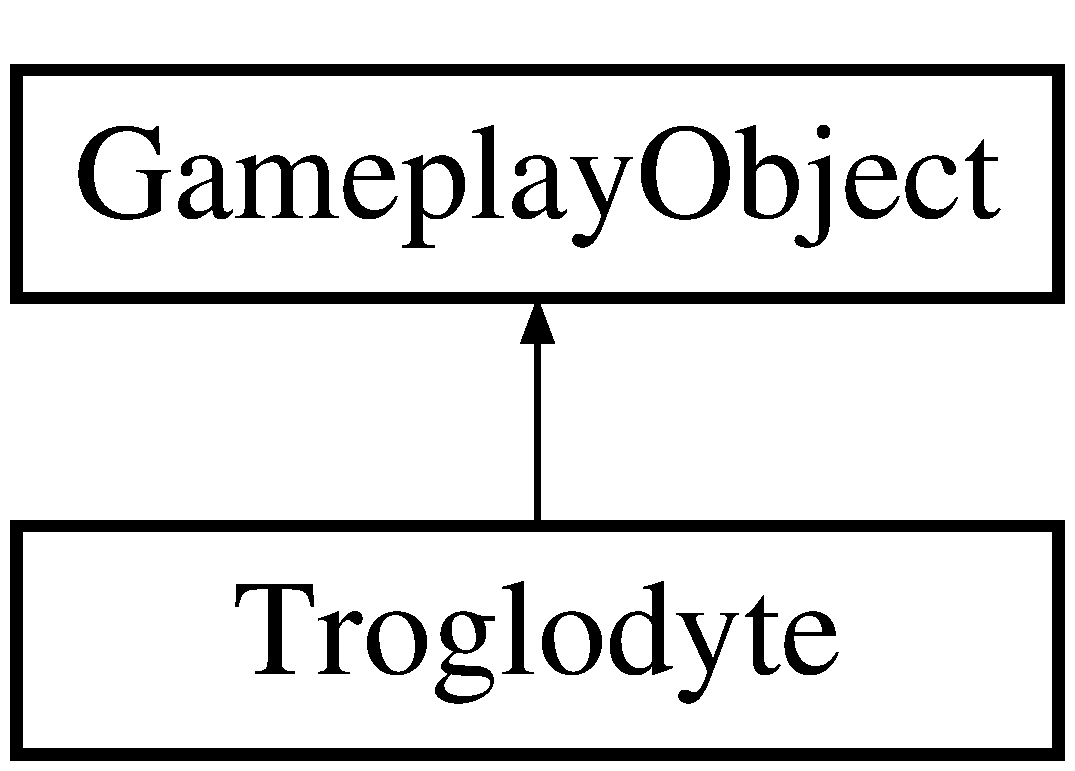
\includegraphics[height=2.000000cm]{dd/d4c/classTroglodyte}
\end{center}
\end{figure}
\subsection*{Public Member Functions}
\begin{DoxyCompactItemize}
\item 
void \hyperlink{classTroglodyte_a8dced6c4c8542fd20eb58e05f4ee96d1}{place} (int \hyperlink{classTroglodyte_aac112a5de7a1929974a0e20b4dc12ed8}{x}, int y)
\item 
void \hyperlink{classTroglodyte_ace39490a0220ea11ca717e479c761e0d}{draw} (Graphics2\-D g)
\end{DoxyCompactItemize}
\subsection*{Private Attributes}
\begin{DoxyCompactItemize}
\item 
int \hyperlink{classTroglodyte_a7ecf207954b0beaba51cd0109f576f5d}{width}
\item 
int \hyperlink{classTroglodyte_aac112a5de7a1929974a0e20b4dc12ed8}{x}
\item 
Color \hyperlink{classTroglodyte_ab8ed3473930390172ebbcfbd130e15ba}{color}
\end{DoxyCompactItemize}


\subsection{Member Function Documentation}
\hypertarget{classTroglodyte_ace39490a0220ea11ca717e479c761e0d}{\index{Troglodyte@{Troglodyte}!draw@{draw}}
\index{draw@{draw}!Troglodyte@{Troglodyte}}
\subsubsection[{draw}]{\setlength{\rightskip}{0pt plus 5cm}void Troglodyte.\-draw (
\begin{DoxyParamCaption}
\item[{Graphics2\-D}]{g}
\end{DoxyParamCaption}
)\hspace{0.3cm}{\ttfamily [virtual]}}}\label{classTroglodyte_ace39490a0220ea11ca717e479c761e0d}


Implements \hyperlink{classGameplayObject_ad0e03d54842aa2bb721648ad702ef350}{Gameplay\-Object}.

\hypertarget{classTroglodyte_a8dced6c4c8542fd20eb58e05f4ee96d1}{\index{Troglodyte@{Troglodyte}!place@{place}}
\index{place@{place}!Troglodyte@{Troglodyte}}
\subsubsection[{place}]{\setlength{\rightskip}{0pt plus 5cm}void Troglodyte.\-place (
\begin{DoxyParamCaption}
\item[{int}]{x, }
\item[{int}]{y}
\end{DoxyParamCaption}
)\hspace{0.3cm}{\ttfamily [virtual]}}}\label{classTroglodyte_a8dced6c4c8542fd20eb58e05f4ee96d1}


Implements \hyperlink{classGameplayObject_ad99f71d67a42e68dad3f923adc8a2699}{Gameplay\-Object}.



\subsection{Member Data Documentation}
\hypertarget{classTroglodyte_ab8ed3473930390172ebbcfbd130e15ba}{\index{Troglodyte@{Troglodyte}!color@{color}}
\index{color@{color}!Troglodyte@{Troglodyte}}
\subsubsection[{color}]{\setlength{\rightskip}{0pt plus 5cm}Color Troglodyte.\-color\hspace{0.3cm}{\ttfamily [private]}}}\label{classTroglodyte_ab8ed3473930390172ebbcfbd130e15ba}
\hypertarget{classTroglodyte_a7ecf207954b0beaba51cd0109f576f5d}{\index{Troglodyte@{Troglodyte}!width@{width}}
\index{width@{width}!Troglodyte@{Troglodyte}}
\subsubsection[{width}]{\setlength{\rightskip}{0pt plus 5cm}int Troglodyte.\-width\hspace{0.3cm}{\ttfamily [private]}}}\label{classTroglodyte_a7ecf207954b0beaba51cd0109f576f5d}
\hypertarget{classTroglodyte_aac112a5de7a1929974a0e20b4dc12ed8}{\index{Troglodyte@{Troglodyte}!x@{x}}
\index{x@{x}!Troglodyte@{Troglodyte}}
\subsubsection[{x}]{\setlength{\rightskip}{0pt plus 5cm}int Troglodyte.\-x\hspace{0.3cm}{\ttfamily [private]}}}\label{classTroglodyte_aac112a5de7a1929974a0e20b4dc12ed8}


The documentation for this class was generated from the following file\-:\begin{DoxyCompactItemize}
\item 
src/\hyperlink{Troglodyte_8java}{Troglodyte.\-java}\end{DoxyCompactItemize}

\chapter{File Documentation}
\hypertarget{GameLogic_8java}{\section{src/\-Game\-Logic.java File Reference}
\label{GameLogic_8java}\index{src/\-Game\-Logic.\-java@{src/\-Game\-Logic.\-java}}
}
\subsection*{Classes}
\begin{DoxyCompactItemize}
\item 
class \hyperlink{classGameLogic}{Game\-Logic}
\end{DoxyCompactItemize}

\hypertarget{GameplayObject_8java}{\section{src/\-Gameplay\-Object.java File Reference}
\label{GameplayObject_8java}\index{src/\-Gameplay\-Object.\-java@{src/\-Gameplay\-Object.\-java}}
}
\subsection*{Classes}
\begin{DoxyCompactItemize}
\item 
class \hyperlink{classGameplayObject}{Gameplay\-Object}
\end{DoxyCompactItemize}

\hypertarget{GameplayObjectsList_8java}{\section{src/\-Gameplay\-Objects\-List.java File Reference}
\label{GameplayObjectsList_8java}\index{src/\-Gameplay\-Objects\-List.\-java@{src/\-Gameplay\-Objects\-List.\-java}}
}
\subsection*{Classes}
\begin{DoxyCompactItemize}
\item 
class \hyperlink{classGameplayObjectsList}{Gameplay\-Objects\-List}
\end{DoxyCompactItemize}

\hypertarget{GameWindow_8java}{\section{src/\-Game\-Window.java File Reference}
\label{GameWindow_8java}\index{src/\-Game\-Window.\-java@{src/\-Game\-Window.\-java}}
}
\subsection*{Classes}
\begin{DoxyCompactItemize}
\item 
class \hyperlink{classGameWindow}{Game\-Window}
\end{DoxyCompactItemize}

\hypertarget{Main_8java}{\section{src/\-Main.java File Reference}
\label{Main_8java}\index{src/\-Main.\-java@{src/\-Main.\-java}}
}
\subsection*{Classes}
\begin{DoxyCompactItemize}
\item 
class \hyperlink{classMain}{Main}
\end{DoxyCompactItemize}

\hypertarget{MapPanel_8java}{\section{src/\-Map\-Panel.java File Reference}
\label{MapPanel_8java}\index{src/\-Map\-Panel.\-java@{src/\-Map\-Panel.\-java}}
}
\subsection*{Classes}
\begin{DoxyCompactItemize}
\item 
class \hyperlink{classMapPanel}{Map\-Panel}
\end{DoxyCompactItemize}

\hypertarget{Order_8java}{\section{src/\-Order.java File Reference}
\label{Order_8java}\index{src/\-Order.\-java@{src/\-Order.\-java}}
}
\subsection*{Classes}
\begin{DoxyCompactItemize}
\item 
class \hyperlink{classOrder}{Order}
\end{DoxyCompactItemize}

\hypertarget{Player_8java}{\section{src/\-Player.java File Reference}
\label{Player_8java}\index{src/\-Player.\-java@{src/\-Player.\-java}}
}
\subsection*{Classes}
\begin{DoxyCompactItemize}
\item 
class \hyperlink{classPlayer}{Player}
\end{DoxyCompactItemize}

\hypertarget{Squadron_8java}{\section{src/\-Squadron.java File Reference}
\label{Squadron_8java}\index{src/\-Squadron.\-java@{src/\-Squadron.\-java}}
}
\subsection*{Classes}
\begin{DoxyCompactItemize}
\item 
class \hyperlink{classSquadron}{Squadron}
\end{DoxyCompactItemize}

\hypertarget{Troglodyte_8java}{\section{src/\-Troglodyte.java File Reference}
\label{Troglodyte_8java}\index{src/\-Troglodyte.\-java@{src/\-Troglodyte.\-java}}
}
\subsection*{Classes}
\begin{DoxyCompactItemize}
\item 
class \hyperlink{classTroglodyte}{Troglodyte}
\end{DoxyCompactItemize}

%--- End generated contents ---

% Index
\newpage
\phantomsection
\addcontentsline{toc}{part}{Index}
\printindex

\end{document}
